% generated by scripts/pkl_to_latex.py
% source PKL : uscan_v1_L8_Ne8_t1_mode-uniform_nmin2_solver-gcg_full_restarts8_iter200_kmax4_tol1em09_U1to20_N20-d03a74da789e.pkl
% scan type  : uscan
% state      : gs
% quantity   : vn-entropy
% requires   : \usepackage{pgfplots} \pgfplotsset{compat=1.18}
% colours match the matplotlib PDF (tab10 cycle)
\definecolor{gmeC0}{HTML}{1F77B4}
\definecolor{gmeC1}{HTML}{FF7F0E}
\definecolor{gmeC2}{HTML}{2CA02C}
\definecolor{gmeC3}{HTML}{D62728}
\definecolor{gmeC4}{HTML}{9467BD}
\definecolor{gmeC5}{HTML}{8C564B}
\definecolor{gmeC6}{HTML}{E377C2}
\definecolor{gmeC7}{HTML}{17BECF}

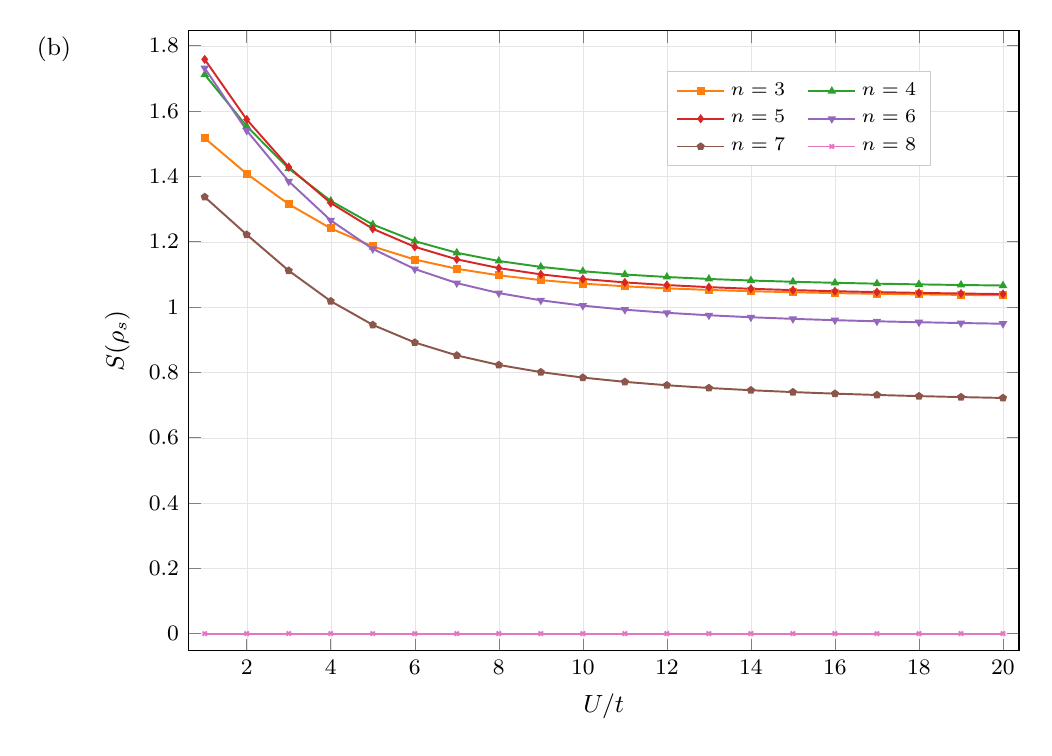
\begin{tikzpicture}
  \begin{axis}[
    width=\columnwidth,
    height=0.78\columnwidth,
    xlabel={$U/t$},
    ylabel={$S(\rho_s)$},
    grid=both,
    grid style={line width=.1pt, draw=gray!20},
    tick label style={font=\footnotesize\rmfamily, /pgf/number format/fixed},
    label style={font=\small\rmfamily},
    scaled ticks=false,
    legend style={font=\scriptsize\rmfamily, draw=gray!40, at={(0.5,1.03)}, anchor=south, /tikz/every even column/.append style={column sep=6pt}},
    legend cell align={left},
    legend columns=2,
    ymin=-0.053,
    ymax=1.846,
    xmin=0.62,
    xmax=20.38,
    legend style={at={(0.735,0.858)}, anchor=center, fill=white},
    after end axis/.append code={\node[anchor=east, font=\small\rmfamily] at (axis description cs:-0.13,0.970) {(b)};},
  ]
    \addplot[color=gmeC1, mark=square*, mark size=1.1pt, line width=0.7pt] coordinates {
        (1,1.517103) (2,1.408053) (3,1.314891) (4,1.24085)
        (5,1.18539) (6,1.145469) (7,1.117161) (8,1.096995)
        (9,1.082401) (10,1.071622) (11,1.06349) (12,1.057229)
        (13,1.052319) (14,1.048402) (15,1.045232) (16,1.042631)
        (17,1.040471) (18,1.03866) (19,1.037125) (20,1.035814)
    };
    \addlegendentry{$n=3$}
    \addplot[color=gmeC2, mark=triangle*, mark size=1.1pt, line width=0.7pt] coordinates {
        (1,1.711623) (2,1.55349) (3,1.424124) (4,1.324964)
        (5,1.252718) (6,1.201737) (7,1.166083) (8,1.140927)
        (9,1.122848) (10,1.109563) (11,1.099579) (12,1.091915)
        (13,1.085919) (14,1.081145) (15,1.077286) (16,1.074125)
        (17,1.071503) (18,1.069304) (19,1.067444) (20,1.065855)
    };
    \addlegendentry{$n=4$}
    \addplot[color=gmeC3, mark=diamond*, mark size=1.1pt, line width=0.7pt] coordinates {
        (1,1.758277) (2,1.57415) (3,1.428348) (4,1.318521)
        (5,1.239514) (6,1.184335) (7,1.146054) (8,1.119204)
        (9,1.099986) (10,1.085902) (11,1.075335) (12,1.06723)
        (13,1.06089) (14,1.055842) (15,1.051759) (16,1.04841)
        (17,1.04563) (18,1.043297) (19,1.04132) (20,1.03963)
    };
    \addlegendentry{$n=5$}
    \addplot[color=gmeC4, mark=triangle*, mark size=1.1pt, mark options={rotate=180}, line width=0.7pt] coordinates {
        (1,1.7316) (2,1.540304) (3,1.384846) (4,1.265194)
        (5,1.177936) (6,1.11636) (7,1.073219) (8,1.042661)
        (9,1.020575) (10,1.004235) (11,0.991865) (12,0.982297)
        (13,0.974752) (14,0.968698) (15,0.963768) (16,0.959698)
        (17,0.956298) (18,0.953427) (19,0.95098) (20,0.948877)
    };
    \addlegendentry{$n=6$}
    \addplot[color=gmeC5, mark=pentagon*, mark size=1.1pt, line width=0.7pt] coordinates {
        (1,1.336964) (2,1.221641) (3,1.11137) (4,1.017946)
        (5,0.945331) (6,0.891397) (7,0.851847) (8,0.822643)
        (9,0.800727) (10,0.783959) (11,0.770878) (12,0.760488)
        (13,0.752099) (14,0.745227) (15,0.739524) (16,0.734736)
        (17,0.730676) (18,0.727201) (19,0.724202) (20,0.721595)
    };
    \addlegendentry{$n=7$}
    \addplot[color=gmeC6, mark=x, mark size=1.1pt, line width=0.7pt] coordinates {
        (1,0) (2,0) (3,0) (4,0)
        (5,0) (6,0) (7,0) (8,0)
        (9,0) (10,0) (11,0) (12,0)
        (13,0) (14,0) (15,0) (16,0)
        (17,0) (18,0) (19,0) (20,0)
    };
    \addlegendentry{$n=8$}
  \end{axis}
\end{tikzpicture}
